\section{Runtime System}\label{sec:runtime-system}
The runtime system of parlallel.es consists of two parts: The public api in the ui-thread that forms the facade and acts as the master for the slaves. The slaves run in background-threads and perform the computations defined by the tasks. Applications are using the facade provided by the master to run functions in a background thread. The master is responsible for spawning the slaves and distributing the work onto these. The runtime system uses by default a fair FIFO thread pool with a constant limit of background-threads initialized with the number of logical processors provided by the hardware\footnote{The api \javascriptinline/navigator.hardwareConcurrency/ provides the logical processor counts on newer browser. A default of 4 is assumed when the api is not available in the used browser}. The thread pool implementation is interchangeable. 

\subsection{Task Roundtrip}
The steps needed to process a single task are shown in \cref{fig:runtime-system}. The application passes the function to execute in a background-thread together with the arguments to pass to the function to the facade that acts as master (1). The master creates a serialized representation of the function call to perform since messaging must be used between the master and slave as implied by the Web Worker programing model. The serialized representation consists of a unique id to the function to call and the arguments with which the function should be called. These information are passed to the slave (2). The slave performs a lookup on the function cache to retrieve the function with the given id (3). The function definition is requested from the master (4, 5), instantiated as a function and registered in the function cache (6) if the function is executed the first time on this slave --- and therefore no registration exists in the function cache. The slave calls the deserialized function with the provided arguments (7) and returns the (structured cloned) result back to the master (8). The master invokes the success handler in the ui-thread to pass the result to the application (9). 

\begin{figure*}
	\centering
	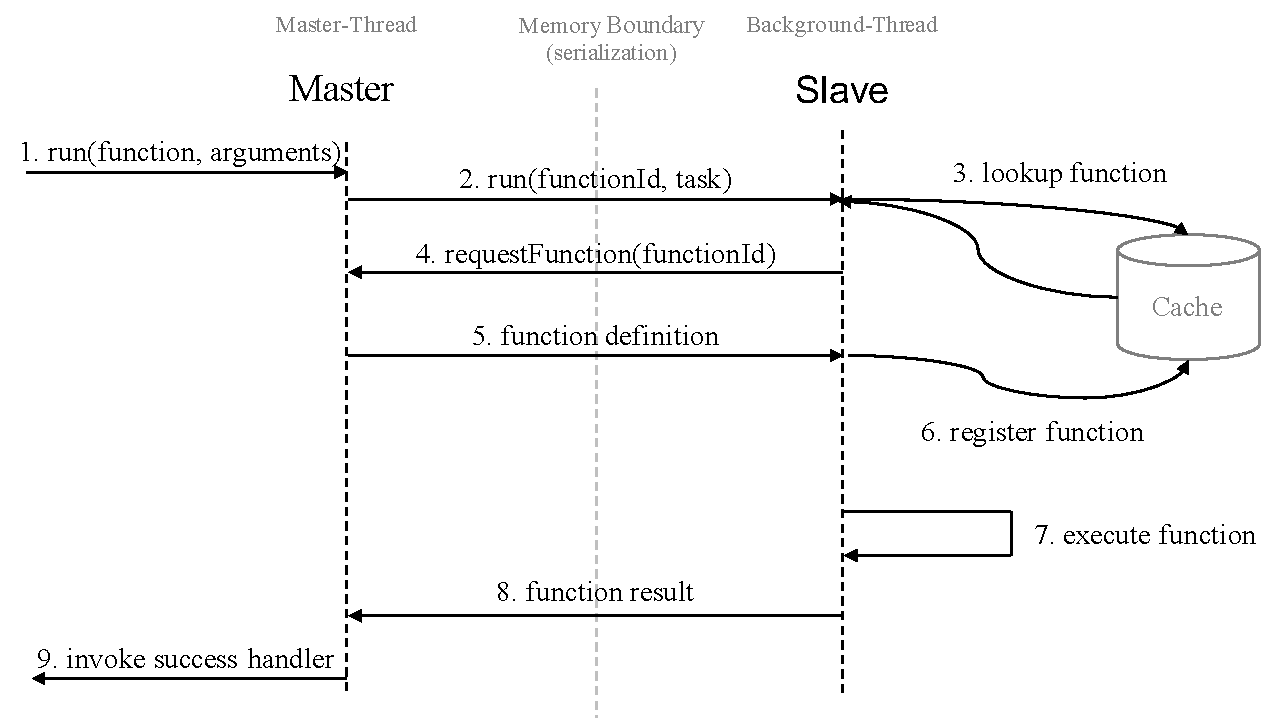
\includegraphics[width=0.8\textwidth]{runtime-system.pdf}

	\caption{Parallel.es Runtime System}
	\label{fig:runtime-system}
\end{figure*}

The caching of the function definitions on the slave have the advantage that performed JIT-optimizations are not thrown away if a task has completed. It is believed that the gain of reusing the JIT-Optimized function outweighs the additional costs caused by the function lookup and additional roundtrip for function retrieval. Especially for frequent but short running tasks. 


\subsection{Limitations}
The current implementation supports the most essential features. However, the implementation currently is missing the support for asynchronous task operations and the NodeJS environment. There are no technical reasons for not supporting either of these features. Adding support for NodeJS requires using a structured clone polyfill as this is not supported by NodeJS.

A further limitation is that tasks can not be started from inside of a task. An efficient implementation supporting task scheduling from inside a task requires a communication channel between all web workers that allows to directly transmit the data to the started background-thread without an additional roundtrip over the ui-thread. However, Web Workers only allow to have a single communication channel. If the support for older browsers is dropped than the feature might be implemented using Shared Workers~\cite[section 4.6.4]{w3cWebWorker}